\subsection{Label Confusion and Error Breakdown}
\label{ssec:label_confusion}
% The MISC annotation guidelines~\cite{miller2003manual,
%   houck2012motivational} lists labels that are known to be easily confused.

%   with each other except between \GI, \QUO, \QUC.

Figure \ref{fig:categorizing_confusion_client} shows the confusion
matrix for the client categorization task. The confusion between \FN
and \CHANGE/\SUSTAIN is largely caused by label imbalance. There are 414 \CHANGE examples that are predicted as \SUSTAIN
and 391 examples vice versa. To further understand their confusion, we
selected 100 of each for manual analysis. We found four broad
categories of confusion, shown in Table
\ref{tbl:c_client_errors}.

\begin{figure}[!h]
\centering
  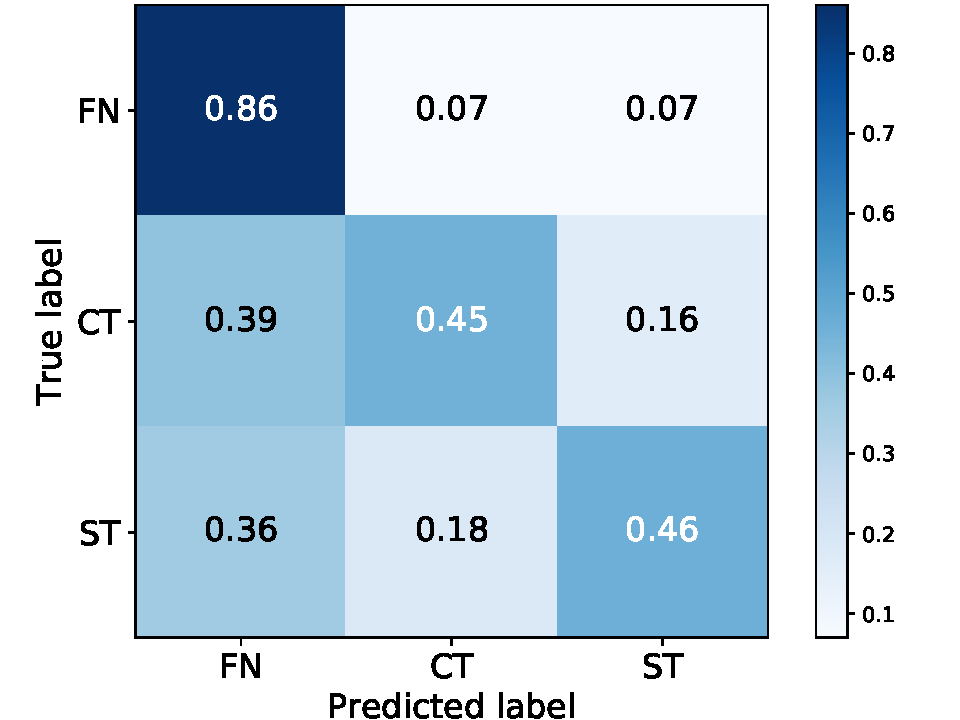
\includegraphics[width=0.50\textwidth]{large_font_categorizing_plabel_confusion_matrix_dev.pdf}
  \caption{\label{fig:categorizing_confusion_client} Confusion matrix for categorizing client codes, normalized by row.}
\end{figure}

\begin{table}[!h]
\caption{Categorization of \CHANGE/\SUSTAIN confusions.The two numbers in the brackets are the count of errors for predicting \CHANGE as \SUSTAIN and vice versa. We exampled 100 examples for each case.}
  \small
  \begin{center}
\begin{tabular}{ll}
  \toprule
  {\bf Category and Explaination}                                                                                                                                                                                                                            & {\bf Client Examples (Gold MISC)}                                                                                                                                         \\\midrule
  \multirow{4}{*}{\parbox{7cm}{Reasoning is required to understand
  whether a client wants to change behavior, even with full context~(50,42) }}                               & \multirow{4}{*}{\parbox{7cm}{T: On a scale of zero to ten how confident are you that you can implement this change? \\C: I don't know, seven maybe (\CHANGE);\\ I have to wind down after work (\SUSTAIN) }} \\
                                                                                                                                                                                                                                                             &                                                                                                                                                                     \\
                                                                                                                                                                                                                                                             &                                                                                                                                                                     \\
                                                                                                                                                                                                                                                             &                                                                                                                                                                     \\\midrule
  \multirow{4}{*}{\parbox{7cm}{Concise utterances which are easy for humans to understand, but missing information such as coreference, zero pronouns~(22,31)}}                                                                                        & \multirow{4}{*}{\parbox{7cm}{I mean I could try it (\CHANGE)\\Not a negative consequence for me (\SUSTAIN) \\I want to get every single second and minute out of it(\CHANGE)}}                                                                                                                                     \\
                                                                                                                                                                                                                                                             & \\
                                                                                                                                                                                                                                                             & \\
                                                                                                                                      & \\\midrule
  \multirow{3}{*}{\parbox{7cm}{Extremely short ($ \leq5 $) or long sentence ($\ge40 $), caused by incorrect turn segementation. ~(21,23)}} & It is a good thing (\SUSTAIN)                                   \\
                                                                                                                                      & Frankly, I hate it (\CHANGE)                                                               \\ & Painful (\CHANGE)                                                                                                                                                    \\ \midrule
  \multirow{2}{*}{\parbox{7cm}{Ambivalent speech, very hard to understand even for human.~(7,4)}}                                     & \multirow{3}{*}{\parbox{7cm}{What if it does n't work I mean what if I can't do it (\SUSTAIN)\\But I can stop whenever I want(\SUSTAIN)}}                                                                                                                            \\
& \\                                                                                                                                                                                                                                                             &                                                                                                                             \\\bottomrule
\end{tabular}
\end{center}
\label{tbl:c_client_errors}
\end{table}

The first category requires more complex reasoning than just surface
form matching. For example, the phrase \example{seven out of ten}
indicates that the client is very confident about changing behavior;
the phrase \example{wind down after work} indicates, in this context,
that the client drinks or smokes after work. We also found that the
another frequent source of error is incomplete information. In a
face-to-face therapy session, people may use concise and effient
verbal communication, with guestures and other body language conveying
information without explaining details about, for example,
coreference.  With only textual context, it is difficult to infer the
missing information. The third category of errors is introduced when
speech is transcribed into text. The last category is about ambivalent
speech. Discovering the real attitude towards behavior change behind
such utterances could be difficult, even for an expert therapist.
% \todo{@Vivek, I found this is interesting but
%   not easy to write in professoinal linguistic term, please help to revise}
%\begin{table}[!htbp]
%\begin{center}
%\setlength{\tabcolsep}{5pt}
%\begin{tabular}{c|c|c}
%\toprule
%Label & Confusion Label Set          & Model2T & Kappa\\
%\midrule
%FA    & \RES, \REC, GI, QUC, QUO, MIA(Structure), MIN(Confront)                \\
%\RES   & FA, \REC, GI, QUC,QUO, MIA(Affirm, Emphasize Control), MIN(Confront)     \\
%\REC   & FA, \RES, GI, QUC,QUO, MIA(Affirm, Emphasize Control), MIN(Confront)   \\
%GI    & FA, \RES, \REC, MIA(ADP), MIN(Confront, Warn, Direct)                \\
%QUC   & FA,\RES, \REC,QUO,MIA(ADW), MIN          \\
%QUO   & FA,\RES, \REC,QUC,MIA(ADW), MIN         \\
%MIA   & FA, \RES, \REC, GI,QUO,QUC, MIN(ADW)                 \\
%MIN   & FA, \RES. \REC,GI,QUC,QUO,MIA(ADP) \\
%\bottomrule
%\end{tabular}
%\end{center}
%\caption{\label{tbl:confusion_guide} Confusing label set for each label from the MISC Annotation guidelines}
%\end{table}
\begin{figure}[!th]
\centering
% \subfloat[Categorizing client codes\label{subfig:c_client}]{
%   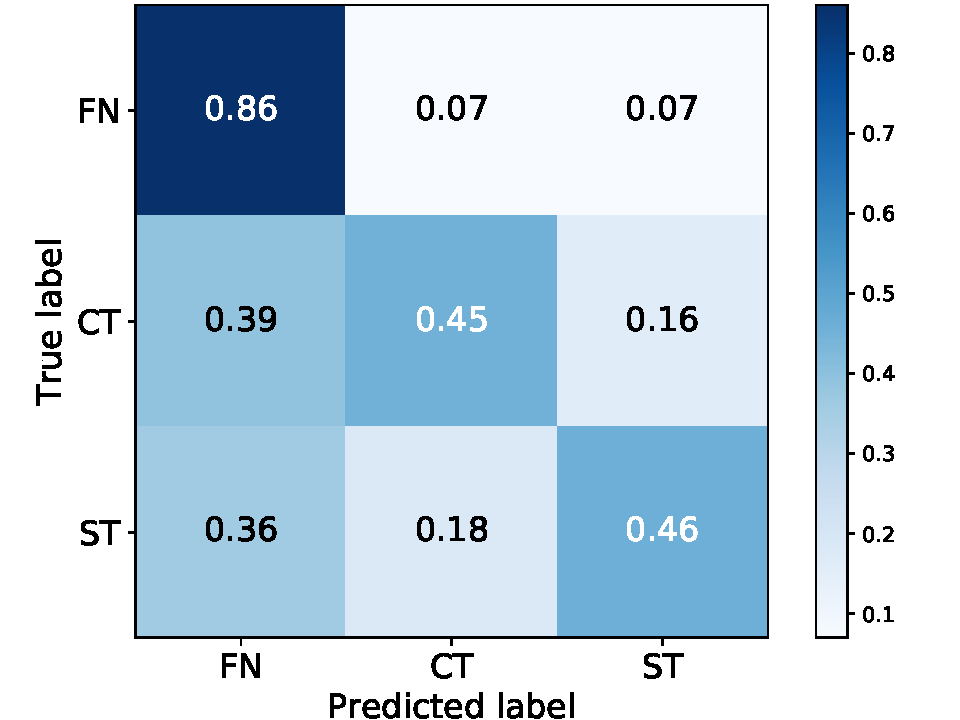
\includegraphics[width=0.24\textwidth]{large_font_categorizing_plabel_confusion_matrix_dev.pdf}
% }
% \subfloat[Forecasting client codes\label{subfig:f_client}]{
%   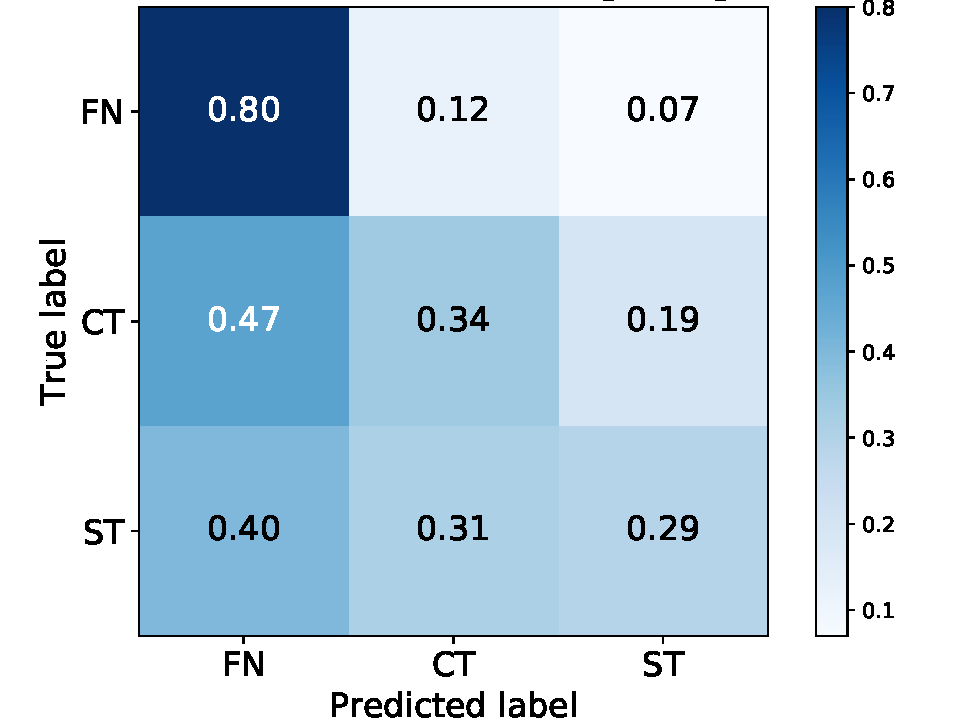
\includegraphics[width=0.24\textwidth, height=3cm]{large_font_forecasting_plabel_confusion_matrix.pdf}
% }

% \subfloat[Categorizing therapist codes\label{subfig:c_therapist}]{
  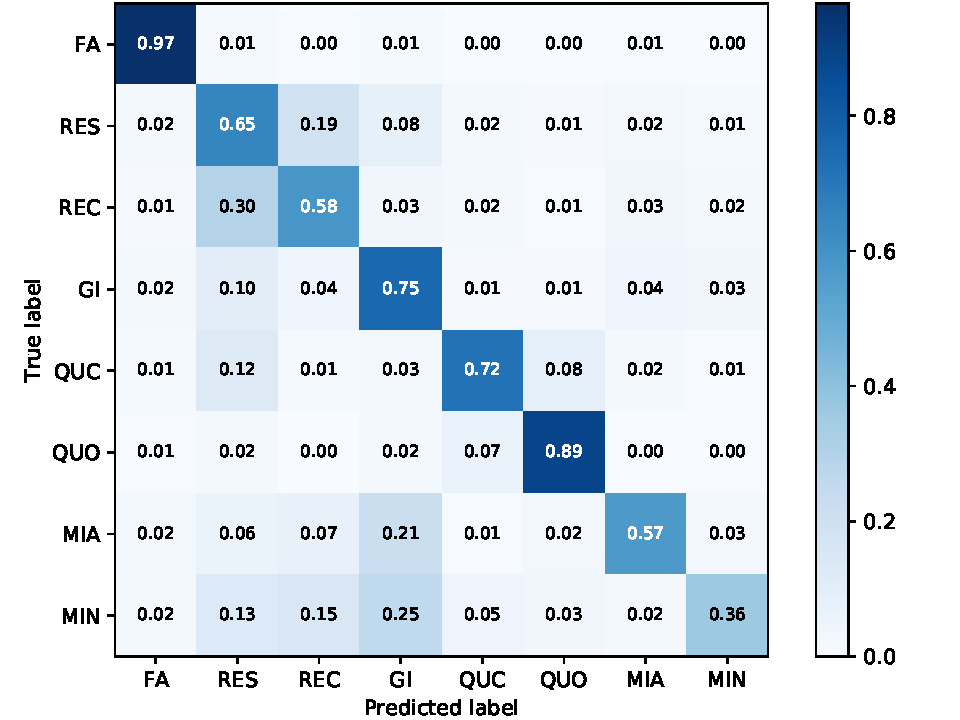
\includegraphics[width=0.90\textwidth]{pred_tlabel_model2_confusion_dev.pdf}
% }
  \caption{\label{fig:categorizing_confusion_therapist} Confusion matrix for categorizing therapist codes, normalized by row.}
\end{figure}

Figures~\ref{fig:categorizing_confusion_client} and~\ref{fig:categorizing_confusion_therapist} show the
label confusion matrices for the best categorization models. We will
examine confusions that are not caused purely by a label being
frequent. We observe a common confusion between
the two reflection labels, \REC and \RES. Compared to the
confusion matrix from \citet{xiao2016behavioral}, we see that our
models show much-decreased confusion here. There are two reason for
this confusion persisting. First, the reflections may require a much
longer information horizon. We found that by increasing the window
size to 16, the overall reflection results improved. Second, we need
to capture richer meaning beyond surface word overlap for
\RES. We found that
complex reflections usually add meaning or emphasis  to
previous client statements using devices such as analogies,
metaphors, or similes rather than simply restating them. % Hence, it requires much other analysis
% more than attention-based word-overlapping.

%
Closed questions (\QUC) and simple reflections (\RES) are known to
be a confusing set of labels. For example, an utterance like
\example{Sounds like you're suffering?} may be both.
%
Giving information (\GI)
is easily confused with many labels because they relate to providing
information to clients, but with different attitudes. The MI adherent
(\MIA) and non-adherent (\MIN) labels may also provide information,
but with supportive or critical attitude that may be difficult to
disentangle, given the limited number of examples.


%\begin{figure}[!htbp]
%\centering
%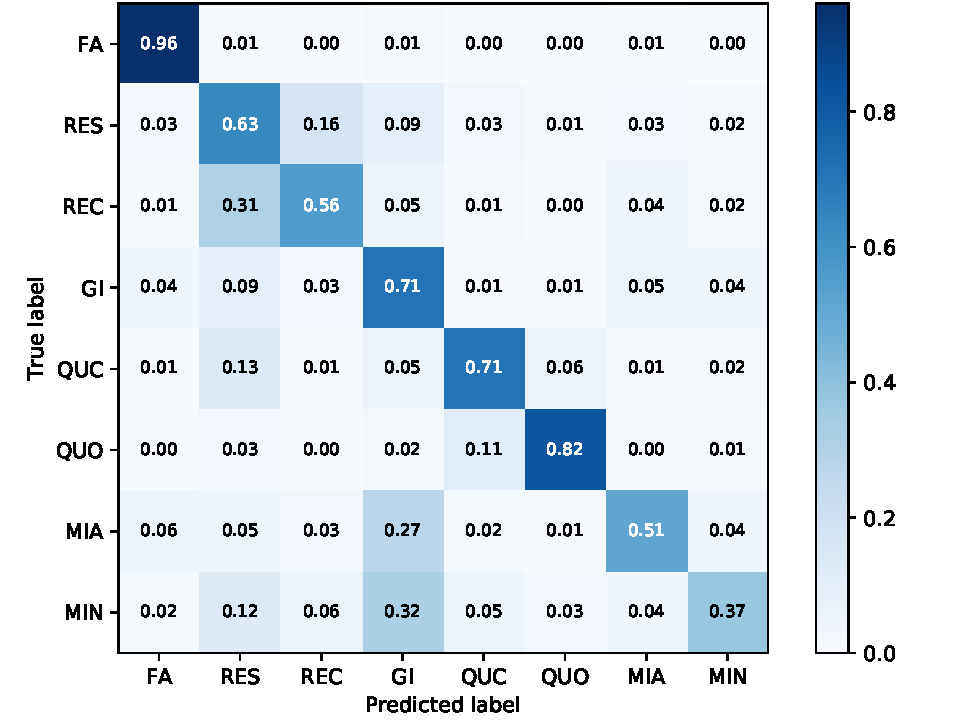
\includegraphics[width=0.5\textwidth]{pred_tlabel_model2_confusion.png}
%\caption{\label{fig:categorizing_t_confusion} Normalized label confusion matrix for categorizing therapist code.}
%\end{figure}

%%% Local Variables:
%%% mode: latex
%%% TeX-master: "../../dissertation-main.ltx"
%%% End:
